\documentclass[article,A4,12pt]{llncs}
\usepackage[T1]{fontenc}
\usepackage{amsmath}
\usepackage{amssymb}
\usepackage{amsfonts}
\usepackage{mathrsfs, bm}

\usepackage{graphicx}
\usepackage{tabularx}
\usepackage{subfig}
\usepackage{epsf,times}
\usepackage{color}
\usepackage{wrapfig}
\usepackage{cases}
\usepackage{multicol}

\usepackage[T1]{fontenc}
%\newcommand{\tmname}[1]{\textsc{#1}}
%\newcommand{\tmop}[1]{\ensuremath{\operatorname{#1}}}
%\newcommand{\tmsamp}[1]{\textsf{#1}}
%\newcommand{\tmtextsc}[1]{{\scshape{#1}}}
%\newcommand{\tmtextsl}[1]{{\slshape{#1}}}
%\newcommand{\tmtexttt}[1]{{\ttfamily{#1}}}

\leftmargin=0.0cm
\oddsidemargin=0.5cm
\evensidemargin=0.5cm
\topmargin=0cm
\textwidth=16.0cm
%\textheight=21.5cm
\textheight=20.0cm
\pagestyle{plain}
\setlength{\columnsep}{20pt}

\def\m{\mathbf{m}}
\def\H{\mathbf{H}}
\def\E{\mathbf{E}}
\newcommand{\vepsi}{{\varepsilon}}
\def\hnorm#1#2{\vert\,#1\,\vert_{#2}}
\newcommand{\R}{{\mathbb R}}
\newcommand{\Sph}{{\mathbb S}}
\def\x{\mathbf{x}}
\def\hvec{\overline{\mathbf{h}}}
\def\evec{\overline{\mathbf{e}}}

\newcommand{ \etal}{\mbox{\emph{et al. }}}

\newcommand\vect[1]{\mbf{#1}}
\newcommand{\mbf}[1]{\mbox{\boldmath$#1$}} 
\newcommand{\RC}[1]{#1 $\times$ #1 $\times$ #1}
\def\um{$\mu$m}
\def\C{$^{\circ}\mathrm{C}$}

\newcommand{\Rmnum}[1]{\expandafter\@slowromancap\romannumeral #1@}

% DEFINITION OF CUSTOM FONT SIZE
\newcommand{\customfontA}{\fontsize{50}{55}\selectfont}
\newcommand{\customfontB}{\fontsize{14.4}{20}\selectfont}
\newcommand{\customfontC}{\fontsize{30}{35}\selectfont}

\DeclareMathAlphabet{\mathpzc}{OT1}{pzc}{m}{it}

\def\clovek#1{\noindent\bgroup\vbox{\noindent#1}\egroup\vskip1em}

% TO INPUT BACKGROUND IMAGE
\usepackage{eso-pic}
\newcommand\BackgroundPic{
\put(0,0){
\parbox[b][\paperheight]{\paperwidth}{
\vfill
\centering
\includegraphics[width=\paperwidth,height=\paperheight]{img/intro-frontpage.png}
%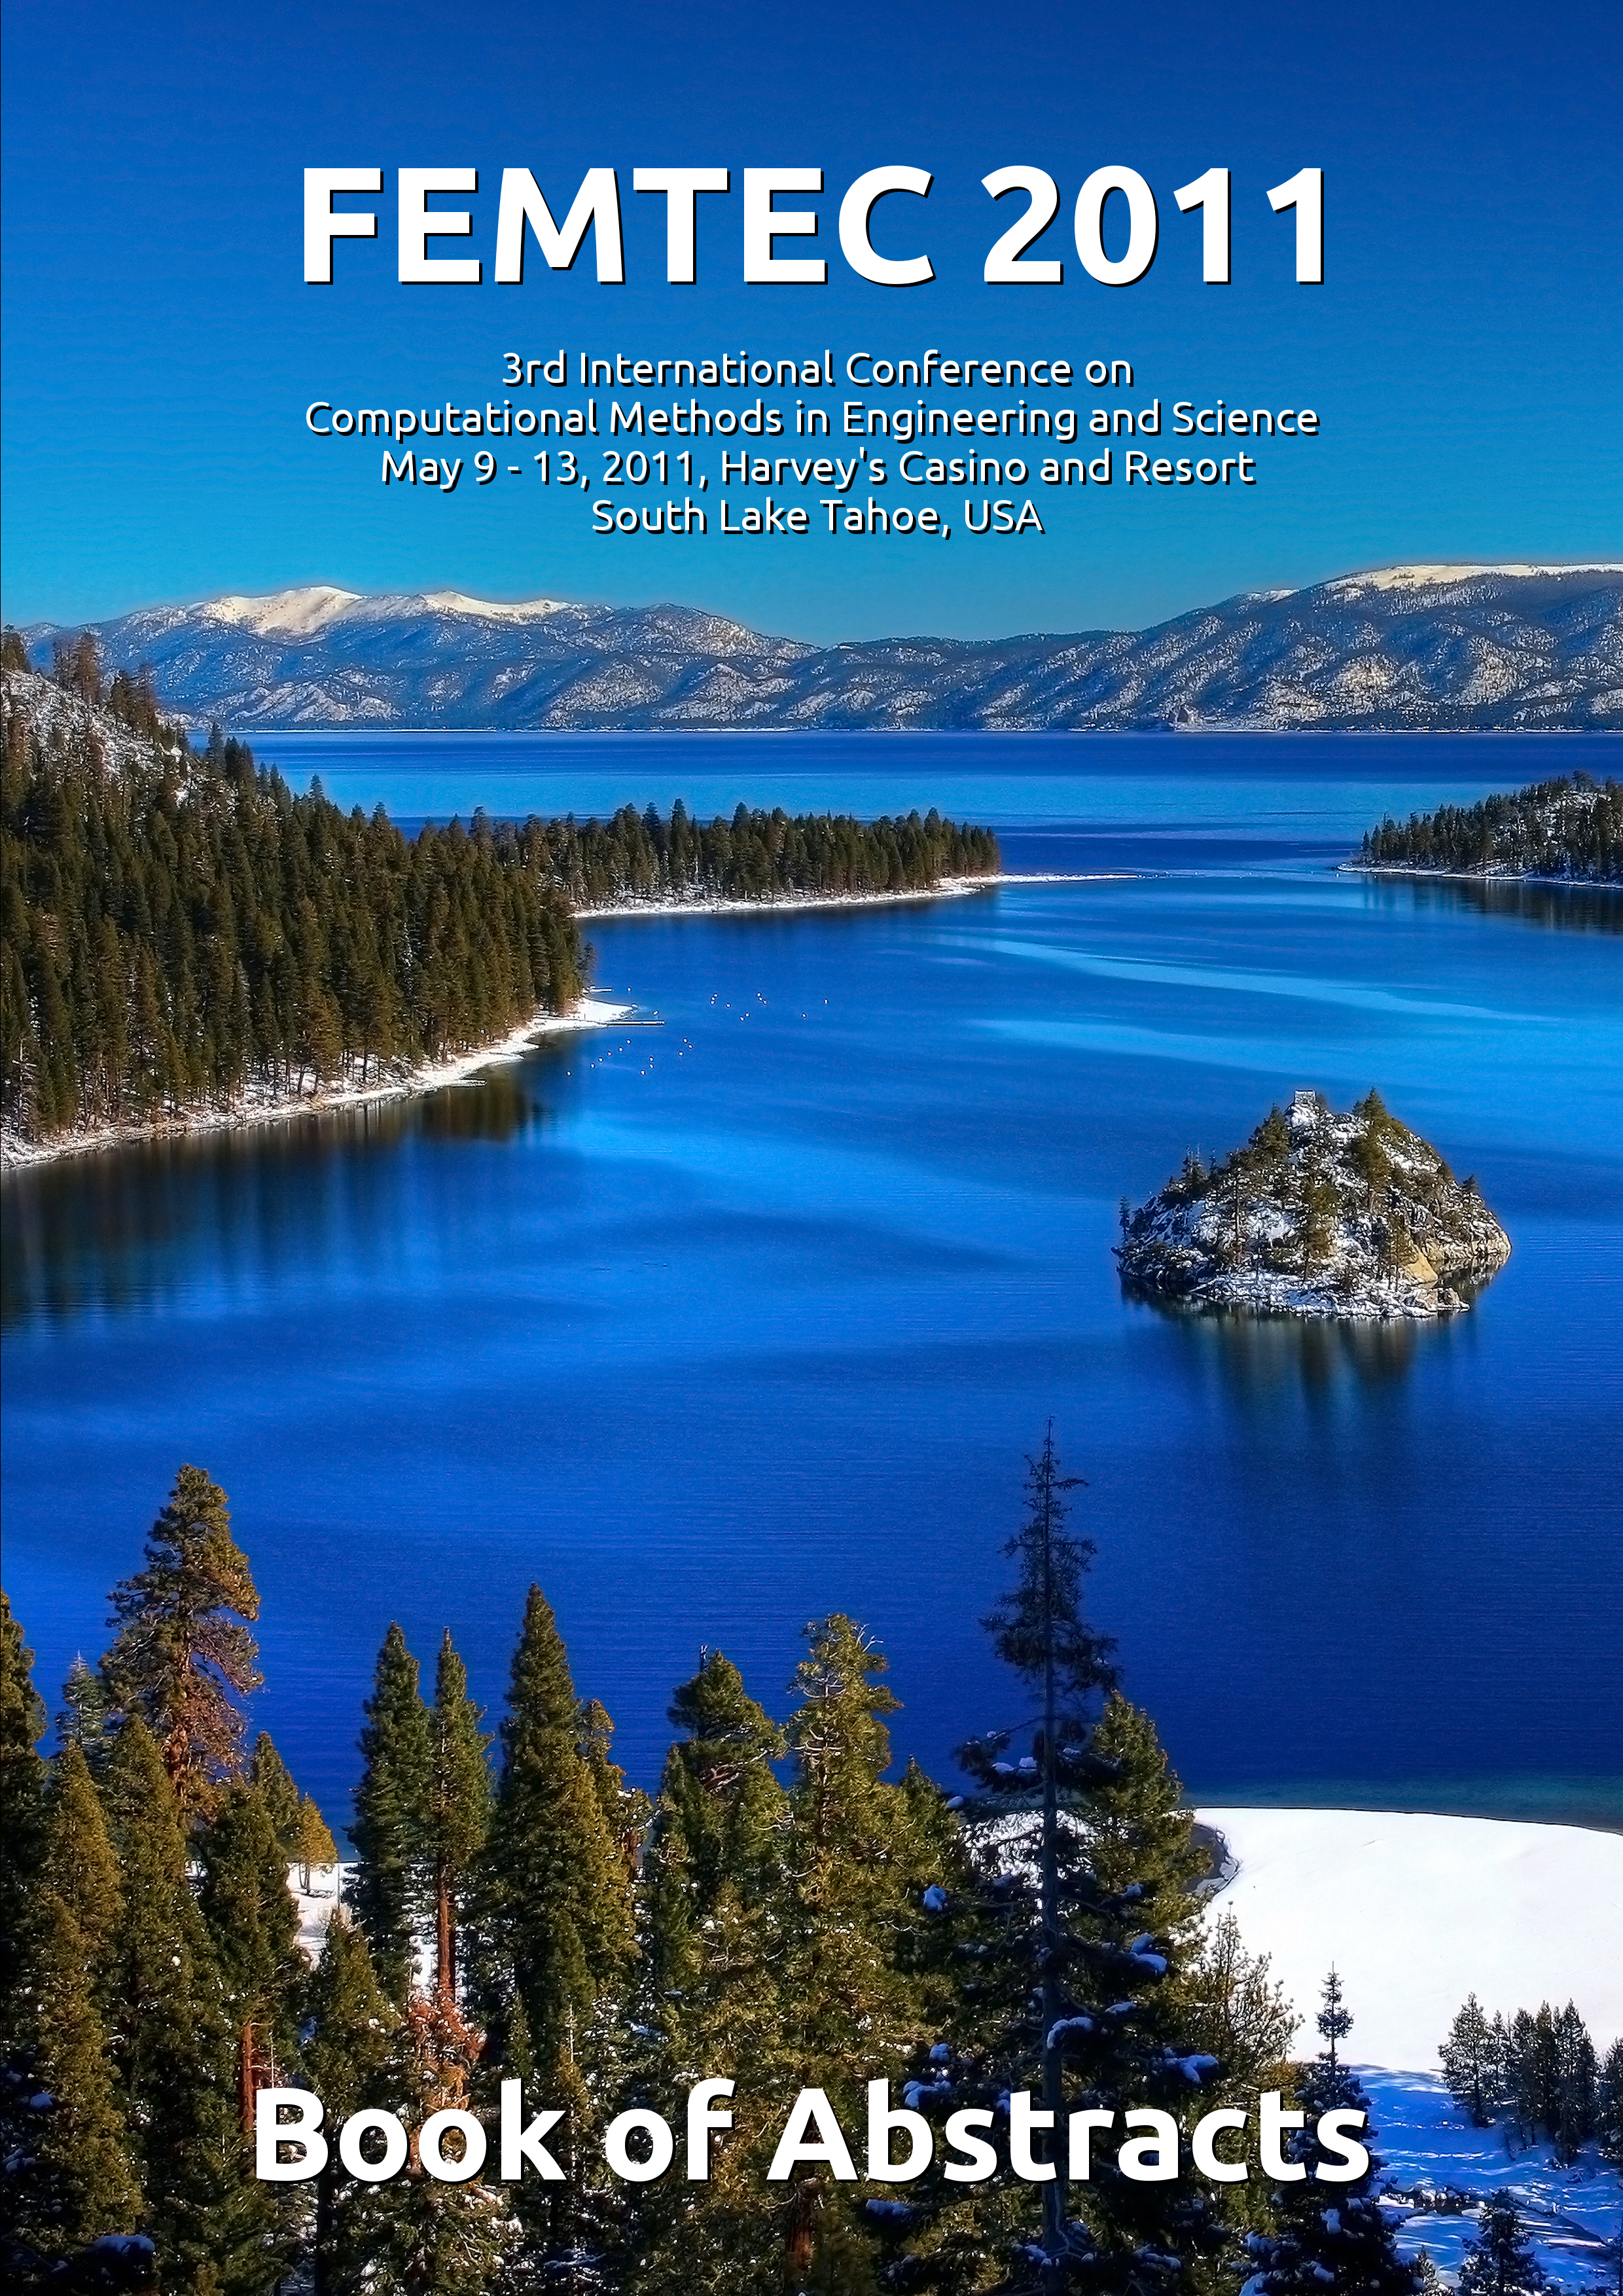
\includegraphics[width=\paperwidth,height=\paperheight]{img/background.jpg}
\vfill
}}}

\begin{document}

% INPUTTING BACKGROUND IMAGE
\AddToShipoutPicture{\BackgroundPic}
\vbox{}
\pagestyle{empty}
\newpage
\textwidth=15.5cm
\ClearShipoutPicture
\newpage

%%%%%%%%%%%%%%%%%%%%%%%%%%%%%%%%%%%%%%%%%%%%%%%%%%%%%%%%%%%%%%%%%%%%%%%%%

\section*{}
\small
\subsection*{About NCLab}
Networked Computing Laboratory (NCLab) is a popular Internet-based framework for 
programming, mathematics, computer modeling, 
and scientific computing. It serves students, instructors, researchers, and the general 
public. NCLab can be used free of charge for personal non-commercial purposes such as 
private hobby or self-education, as well as for individual non-funded academic research.
All other use is subject to {\bf purchasing a license} for a symbolic fee. The fees are as low as 
\$1 per user per month for educational use, and they are used to support the development 
and operational expenses. NCLab is a product of FEMhub Inc. The name "NCLab" is 
registered with the U.S. Patent and Trademark Office (USPTO) under Trademark No. 85420518.

\subsection*{Terms of Use and Pricing}
More details on purchasing a license and using NCLab are provided in the online documents 
{\bf Pricing} and {\bf Terms of Use} that are accessible from NCLab's home page 
{\tt http://nclab.com}.

\subsection*{Contact Information}
General inquiries: {\tt info@femhub.com}\\
Sales: {\tt sales@femhub.com}\\
NCLab support: {\tt support@nclab.com}\\
Agros \& Hermes support: {\tt support@femhub.com}\\
Web page: {\tt http://femhub.com}\\
{Physical address}\\
FEMhub Inc.\\
5490 Twin Creeks Dr.\\
Reno, NV 89523

\subsection*{About This Publication}
This publication can be copied and distributed without any restrictions
as long as reference to NCLab and FEMhub Inc. is preserved.

\subsection*{Acknowledgement}
This publication was created with the help of numerous freely 
available web resources and tutorials related to Python, Scipy,
Numpy, Pylab, Matplotlib, Sympy and other projects.

\normalsize

\newpage
%{\ }
\setcounter{tocdepth}{2}
\tableofcontents
%\pagestyle{plain}

\newpage

\pagestyle{plain}
\setcounter{page}{1}

%%%%%%%%%%%%%%%%%%%%%%%%%%%%%%%%%%%%%%%%%%%%%%%%%%%%%%%%%%%%%%%%%%%%%%%%%


\section{Introduction}

The advantage of simple calculators, such as the one shown in Fig. \ref{fig:xcalc}
is that they only have a few functions, and thus can be operated using a few buttons.

\begin{figure}[!ht]
\begin{center}
\includegraphics[width=0.4\textwidth]{img/xcalc.png}
\end{center}
%\vspace{-2mm}
\caption{Simple calculator.}
\label{fig:xcalc}
\end{figure}
\noindent
Compared to this calculator, NCLab provides an enormous functionality 
that would require thousands and thousands of buttons. So instead of buttons,
in NCLab we use simple commands to get the results we want. The language used 
to talk to NCLab is called Python. Using Python is very intuitive, 
as we shall see in a moment.

\section{Launching a Python Project}

Begin with clicking on the File Manager icon, which launches the File 
Manager. Next go to the menu Project in the upper-left corner. There go 
through the submenu New to Python and click. This will lanuch a new Python 
project, as illustrated in Fig. \ref{fig:python}. The same can be achieved
by clicking on the icon Programming. In the menu that appears, click on 
Python. 

\newpage

\begin{figure}[!ht]
\begin{center}
\includegraphics[width=\textwidth]{img/python.png}
\end{center}
%\vspace{-2mm}
\caption{Python project.}
\label{fig:python}
\end{figure}
\noindent
For now we will be using Python for simple math operations only,
but you could start writing an advanced Python program right 
here if you wanted. An introduction to the Python programming 
language is the subject of another NCLab tutorial.

Before we begin, it is a good idea to save your project under some 
name. This is done through the menu File and submenu Save. For 
now we can save the project in the base folder. Later you can create 
a new folder through the File Manager's menu Folder, and drag there
the project by mouse, to keep your data organized.

\section{Cloning Displayed Projects}

All examples that we are going to work with in the following are also available 
as Displayed Projects. This means that you can clone them by going to the
File Manager's Project menu and clicking on {\em Clone}. This will launch 
a window with many displayed projects from various areas of programming,
math and computing. Look for projects titled such as "Math - Tutorial - 1 - Simple Arithmetic",
"Math - Tutorial - 2 - Commutative, Associative and Distributive Laws", etc.
After you locate a project that you would like to clone, click on it,
and then click on the button "Clone" at the bottom of the window. This will
create exact copy of that project in your account, and you can open it 
by clicking on it in the File Manager. You can change the project in any way 
you like, the changes will not affect the original Displayed Project. 

\section{Simple Arithmetic}

Let's say that we have not cloned the displayed project "Math - Tutorial - 1 - Simple Arithmetic"
and instead, we prefer to start from scratch.
So your project contains a single {\em input cell}. Let's write 
something simple into it, for example "1 + 2", and click 
the link "run" right under the input cell. This sends a request to 
the cloud, it is processed there, and an answer comes back instantly. 
It is displayed in a new (yellow) {\em output cell}, as shown in 
Fig. \ref{fig:1p3}.

\newpage

\begin{figure}[!ht]
\begin{center}
\includegraphics[width=\textwidth]{img/1p2.png}
\end{center}
%\vspace{-2mm}
\caption{Evaluating the expression "1+2".}
\label{fig:1p3}
\end{figure}
\noindent
\noindent
In addition to input and output cells, you can use {\em text cells}
to keep your project commented. This is strongly recommended. In
order to add a new text cell above the input cell, click into
the input cell, and then in menu Edit choose "New text cell above
active cell". A new text cell appears, asking you to click there to
edit its contents. Do so, and write, for example, "**Adding numbers**".
The double stars are used to make a text between them bold face. 
Then click on the link "save" right under the text cell. The result 
is shown in Fig. \ref{fig:1p3r}.

\newpage


\begin{figure}[!ht]
\begin{center}
\includegraphics[width=\textwidth]{img/1p2r.png}
\end{center}
%\vspace{-2mm}
\caption{New descriptive text cell was added above the input cell.}
\label{fig:1p3r}
\end{figure}
\noindent
\noindent
If you like, you can click back into the input cell, change 
the numbers, and click the "run" link under the cell again. 
This will send a new request to the cloud and after the answer 
comes back, it is displayed in the existing output 
cell. 

Let's continue by creating a new empty input cell. To do this, click 
on the "add" below the last input cell. The new input cell will appear below the yellow 
output cell (it will never be placed between an input cell and its 
result). In there, we can experiment with other arithmetic operations 
including subtraction (try for example "5 - 3"), multiplication 
(try for example "3.21 * 7.45"). The results are shown in Fig. \ref{fig:1p3r2}.

\newpage

\begin{figure}[!ht]
\begin{center}
\includegraphics[width=\textwidth]{img/1p2r2.png}
\end{center}
%\vspace{-2mm}
\caption{Subtraction and multiplication.}
\label{fig:1p3r2}
\end{figure}
\noindent
At this point we may go to menu Edit and click on 
"Remove all output" -- this will free up some space.\\

\noindent
{\em BEWARE - Division of Two integers Always is an Integer}\\

Numbers such as "12" or "5" are integers. In Python, as well as 
in other major programming languages, the {\bf result of division of 
two integers always is an integer}. This means that anything beyond 
the decimal point in the result is erased! Let us see this in reality:

\newpage
\begin{figure}[!ht]
\begin{center}
\includegraphics[width=\textwidth]{img/div1.png}
\end{center}
%\vspace{-2mm}
\caption{Division of two integers always is an integer \& two ways to make division safe.}
\label{fig:div1}
\end{figure}
\noindent
Fig. \ref{fig:div1} shows that evaluating simply 12/5 leads to a wrong result. An easy fix is 
to convert one of the numbers into a float by appending a decimal point to it. Still
another way, also shown in  Fig. \ref{fig:div1}, is to convert one of the numbers into a float 
via the function {\tt float()}. The latter approach works even for the division of variables "a/b"
where one may not know exactly whether they are integers or floats. Whenever at least 
one of the numbers if float, the result is a float. \\

\noindent
If you are a mathematician -- yes, you are right. we forgot to discuss division by zero. 
It is useful to see how NCLab reports errors, so let's do it!

\newpage
\begin{figure}[!ht]
\begin{center}
\includegraphics[width=\textwidth]{img/divzero.png}
\end{center}
%\vspace{-2mm}
\caption{Error is reported when dividing by zero.}
\label{fig:divzero}
\end{figure}
\noindent
Since the error message in Fig. \ref{fig:divzero} mentioned modulo, we added there one more 
input cell demonstrating how modulo is done -- using the \% symbol.

\section{Commutative, Associative and Distributive Laws}

The validity of these laws can be verified easily on examples. One just enters
a code similar to 

\begin{verbatim}
a = 2
b = 3
print "a + b =", a + b
print "b + a =", b + a
\end{verbatim}
and clicks on the link "run" under the input cell. The output 
is shown in Fig. \ref{fig:commut}. 

\begin{figure}[!ht]
\begin{center}
\includegraphics[width=0.6\textwidth]{img/commut.png}
\end{center}
\vspace{-4mm}
\caption{Commutative Law holds!}
\label{fig:commut}
%\vspace{-6mm}
\end{figure}




\section{List of Elementary Functions}

In order to calculate square roots, exponentials, sins, cosins, tangents, and all other 
simple functions, the best way is to import Numpy as shown in Fig. \ref{fig:fns}. Numpy 
is a standard Python library for numerical computations.

\begin{figure}[!ht]
\begin{center}
\includegraphics[width=\textwidth]{img/fns.png}
\end{center}
\vspace{-4mm}
\caption{Importing Numpy and using elementary functions.}
\label{fig:fns}
%\vspace{-6mm}
\end{figure}

\newpage
\noindent
Elementary functions that one can import from Numpy include:\\

%{\small
\begin{center}
\begin{tabular}{|l|l|}
\hline
abs($x$) &  absolute value of $x$\\
arccos($x$) &  inverse cosine of $x$ \\
arccosh($x$) &  inverse hyperbolic cosine of $x$ \\
arcsin($x$) & inverse sine of $x$ \\
arcsinh($x$) & inverse hyperbolic sine of $x$ \\
arctan($x$) & inverse tangent of $x$ \\
arctanh($x$) & inverse hyperbolic tangent of $x$ \\
arctan2($x_1$, $x_2$) & arc tangent of $x_1/x_2$ choosing the quadrant correctly \\
cos($x$) & cosine of $x$ \\
cosh($x$) & hyperbolic tangent of $x$ \\
exp($x$) & $e^x$ \\
log($x$) & natural logarithm of $x$ \\
pow($a$, $b$) & $a^b$ (same as "a**b")\\
sin($x$) & sine of $x$ \\
sinh($x$) & hyperbolic sine of $x$ \\
sqrt($x$) & square root of $x$ \\
tan($x$) & tangent of $x$\\
tanh($x$) & hyperbolic tangent of $x$ \\
\hline
\end{tabular}
\end{center}
%}
\vspace{4mm}
\noindent
For a complete overview of functions provided by Numpy we recommend the 
web page \\ {\tt http://www.scipy.org/Numpy\_Functions\_by\_Category}.







\end{document}
